%
% File acl2016.tex
%
%% Based on the style files for ACL-2015, with some improvements
%%  taken from the NAACL-2016 style
%% Based on the style files for ACL-2014, which were, in turn,
%% Based on the style files for ACL-2013, which were, in turn,
%% Based on the style files for ACL-2012, which were, in turn,
%% based on the style files for ACL-2011, which were, in turn, 
%% based on the style files for ACL-2010, which were, in turn, 
%% based on the style files for ACL-IJCNLP-2009, which were, in turn,
%% based on the style files for EACL-2009 and IJCNLP-2008...

%% Based on the style files for EACL 2006 by 
%%e.agirre@ehu.es or Sergi.Balari@uab.es
%% and that of ACL 08 by Joakim Nivre and Noah Smith

\documentclass[11pt]{article}
\usepackage{acl2016}
\usepackage{times}
\usepackage{url}
\usepackage{latexsym}

%% not part of the template

\usepackage{graphicx}
\usepackage{bm}
\usepackage{multirow}
\usepackage{pifont}
\usepackage{amsmath} 
\usepackage{amsthm}
\usepackage{algorithm}
\usepackage{algpseudocode}
\usepackage{varwidth}
\newcommand{\cmark}{\ding{51}}
\newcommand{\xmark}{\ding{55}}
\newtheorem{theorem}{Theorem}
\newtheorem{example}{Example}
\algnewcommand{\LeftComment}[1]{\Statex \(\triangleright\) #1}

\aclfinalcopy % Uncomment this line for the final submission
%\def\aclpaperid{***} %  Enter the acl Paper ID here

%\setlength\titlebox{5cm}
% You can expand the titlebox if you need extra space
% to show all the authors. Please do not make the titlebox
% smaller than 5cm (the original size); we will check this
% in the camera-ready version and ask you to change it back.

\newcommand\BibTeX{B{\sc ib}\TeX}

%\title{Named Entity Recognition Using FOFE}
\title{FOFE-based Deep Neural Networks for Entity Discovery and Linking}

\author{Mingbin Xu, Nargiza Nosirova, Kelvin Jiang, Feng Wei, Hui Jiang \\
	Department of Electrical Engineering and Computer Science \\
	York University,  4700 Keele Street, Toronto, Ontario, M3J 1P3, Canada\\
	{\tt \{xmb,nana,kelvin,fwei,hj\}@eecs.yorku.ca}
}

\date{}

\begin{document}
\maketitle

\begin{abstract}
In this paper, we have studied a novel deep learning method for both mention detection and Entity Linking. Our methods rely on the recent fixed-size ordinally forgetting encoding (FOFE) method to fully encode each sentence fragment and its left/right contexts into a fixed-size representation. Afterwards, a simple feedforward neural network is used to reject or predict entity label for each individual fragment for mention detection and to compute similarity scores with Freebase nodes in the candidate list for entity linking. Experimental results in the 2017 KBP trilingual EDL track have shown that these methods have achieved strong results in both mention detection and entity linking.
\end{abstract}

\section{Introduction}

In this paper, we describe the main techniques used to build our entity discovery and linking systems for the KBP2017 trilingual entity discovery and linking (EDL) track. 
The EDL task requires to detect named
entities of five different types (PER, LOC, ORG, GPE, FAC) 
and their nominal mentions in the raw text
of three languages (English, Chinese and Spanish)
and further link each detected mention to the corresponding
node in an existing knowledge base,
namely Freebase. For NIL mentions that do not exist
in the knowledge base, the EDL system needs to
cluster all NIL mentions and assign a unique ID to
each NIL mention cluster.

In this paper, we have studied a novel deep learning model for both mention detection (MD) and Entity Linking. Our methods rely on the recent fixed-size ordinally forgetting encoding (FOFE) method to fully encode any variable-length text into a fixed-size representation without losing information. 
Experimental results in the 2017 KBP trilingual EDL track have shown that these methods have achieved the strong results in both mention detection and entity linking.

\begin{figure*}[t]
\centering
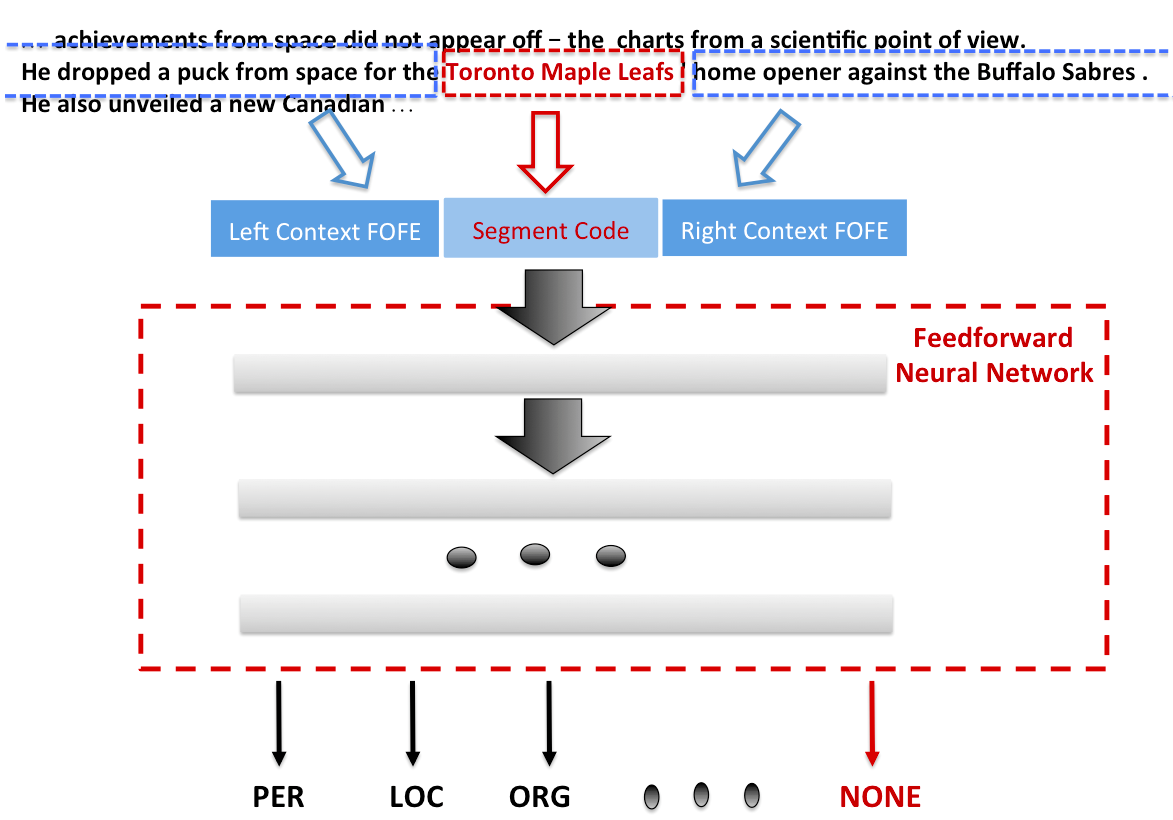
\includegraphics[width=0.75\linewidth]{Figure-Diagram.png}
\caption{Illustration of the local detection approach for NER using FOFE codes as input and a feedforward neural network as model. The window currently examines the fragment of {\it Toronto Maple Leafs}. The window will scan and scrutinize all fragments up to $K$ words. }
\label{Fig:FOFE-NER-diagram}
\end{figure*}

\section{Preliminary: Fixed-size Ordinally Forgetting Encoding (FOFE) }

In this section, we will first briefly review the FOFE technique used in our Entity Discovery and Linking (EDL) system.

A feed-forward neural network (FFNN) is a fast and powerful computation model. 
However, it requires to use fixed-size inputs and 
lacks the ability to capture long-term dependency in sequences. 
Because most NLP problems involve variable-length sequences of words, 
RNNs/LSTMs are more popular than regular feedforward NNs in dealing with these problems. 
The simple encoding method, called Fixed-size Ordinally Forgetting Encoding (FOFE), 
originally proposed in \cite{zhang2015fixed}, nicely overcomes the limitations of deep FNNs because it 
can uniquely encode a variable-length sequence of words into a fixed-size representation without losing information. 

Given a vocabulary $V$ consisting of $|V|$ distinct words, each word can be represented by a one-hot vector. 
FOFE mimics bag-of-words (BOW) but incorporates a forgetting factor to capture positional information.
It encodes any variable-length sequence composed of words in $V$. 
Let $S = {w_1, w_2, w_3, ... , w_T}$ denote a sequence of $T$ words from $V$, 
and $\bm{e_t}$ be the one-hot vector of the $t$-th word in $S$, where $1 \leq t \leq T$.
The FOFE of each partial sequence $\bm{z_t}$ from the first word to the $t$-th word is recursively defined as:
\begin{equation}
\bm{z_t}=
\begin{cases}
\bm{0}, & \text{if}\ t = 0 \\
\alpha \cdot \bm{z_{t - 1}} + \bm{e_t}, & \text{otherwise}
\end{cases}  \label{eq_FOFE_formula}
\end{equation}
where the constant $\alpha$ is called the forgetting factor, and it is chosen between $0$ and $1$ exclusively. 
Evidently, the size of $\bm{z_t}$ is $|V|$, and it is irrelevant to the length of the original sequence, $T$.
According to \cite{zhang2015fixed}, FOFE is capable of uniquely encoding any sequence of arbitrary length, serving as a fixed-size but theoretically lossless representation for any sequence.

\section{Entity Discovery and Mention Detection}

In this work, we have used a new FOFE-based local detection approach to build our systems for 
entity discovery and mention detection, and then we have studied on how to use multi-task learning and model ensemble to further improve the performance. 

\subsection{FOFE-based Models for Named Entity Recognition and Mention Detection}

Our systems, called  \textbf{FOFE-NER} hereafter, 
are motivated by the way how a human actually infers whether a word segment in text is an entity or mention. 
To a large extent, the meaning and spelling of the underlying fragment 
are both informative to distinguish named entities from the rest of the text. 
Context plays a very important role in NER or mention detection 
when it involves multi-sense words/phrases or out-of-vocabulary (OOV) words. 
As shown in Figure \ref{Fig:FOFE-NER-diagram}, our proposed \textbf{FOFE-NER} method examines all possible fragments in text (up to a certain length) one by one. For each fragment, it uses the FOFE method to fully encode the underlying fragment itself, its left context and right context into fixed-size representations, which are in turn fed to a multi-layer feedforward neural network to predict 
whether the current fragment is a valid entity mention (displaying NONE in the case it is not), as well as its correct entity type. This method is appealing because the FOFE codes serve as a theoretically lossless representation of the hypothesis. Since it is full contexts, the multi-layer neural networks are used as a universal approximator to map from text to the entity labels. 

In this work, we use FOFE to explore both word-level and character-level features for each fragment and its contexts.
\textbf{FOFE-NER} generates several word-level features for each fragment hypothesis and its left and right contexts: 
i) Bag-of-word vector of the fragment; ii) FOFE code for left context including the fragment; iii) FOFE code for left context excluding the fragment; iv) FOFE code for right context including the fragment; v) FOFE code for right context excluding the fragment.
On top of the above word-level features, we also augment character-level features for the underlying segment hypothesis to further model its morphological structure: i) Left-to-right FOFE code of the character sequence of the underlying fragment; ii) Right-to-left FOFE code of the character sequence of the underlying fragment.

Evidently, the above \textbf{FOFE-NER} model will take each sentence of words, $S = [w_1, w_2, w_3, ..., w_m]$, as input, and examine all continuous sub-sequences $[w_i, w_{i+1}, w_{i+2}, ..., w_{j}]$ up to $n$ words in $S$ for  possible entity types. All sub-sequences longer than $n$ words are considered as non-entity in this work. 

When we train the model, based on the entity labels of all sentences in the training set, we generate many sentence fragments up to $K$ words. These fragments fall into three categories: i) Exact-match with an entity label, e.g., the fragment  ``{\it Toronto Maple Leafs}'' in the previous example; ii) Partial-overlap with an entity label, e.g., ``{\it for the Toronto}''; iii) Disjoint from all entity labels, e.g. ``{\it from space for}''.
For all exact-matched fragments, we generate the corresponding outputs based on the types of the matched entities in the training set. For both partial-overlap and disjoint fragments, we introduce a new output label, {\bf NONE}, to indicate that these fragments are not a valid entity. Therefore, the output nodes in the neural networks contains all entity types plus a rejection option denoted as {\bf NONE}.

\begin{figure*}[t]
\centering
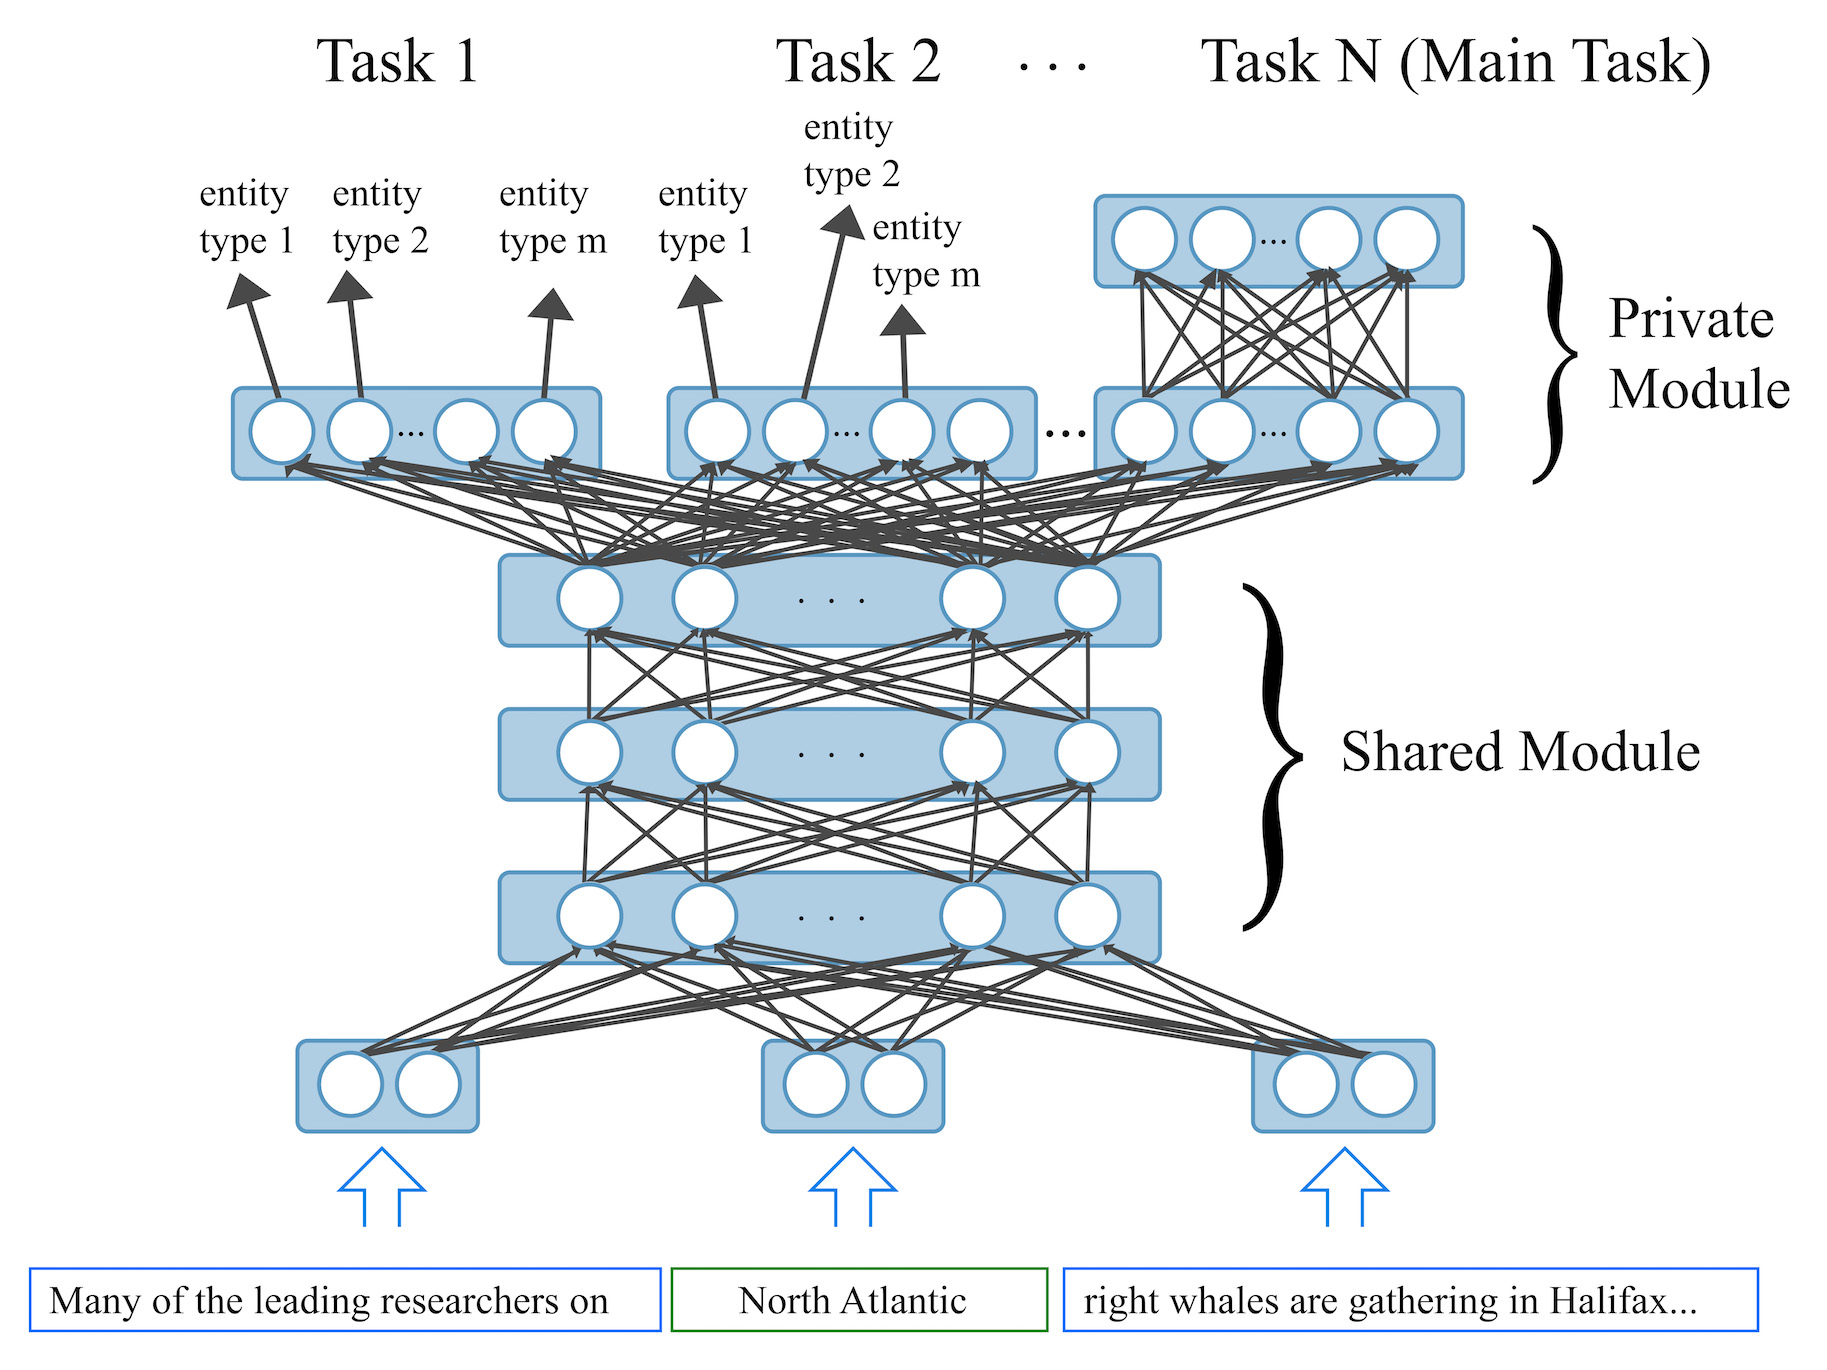
\includegraphics[width=0.8\linewidth]{MTL-method.jpg}
\caption{An illustration of the multi-task feedforward neural network approach for NER using FOFE codes as input. The window currently examines the fragment of {\it North Atlantic}.}
\label{Fig:FOFE-MTL-NER-diagram}
\end{figure*}

\subsection{Multi-Task Learning}

Recently, Multi-task Learning (MTL) has been the centre of a lot of attention. The main idea of MTL lies in concurrently learning a task alongside related (auxiliary) tasks by using a shared representation. Much of the work done in MTL was initiated by \cite{Caruana:1997:ML:262868.262872}. 
His definition of a related task is one that gives the main task a higher performance when trained together as opposed to training it on its own. He also proposes to share features and hidden modules for better performance. Such techniques have been used and confirmed in many studies \cite{Maurer:2016:BMR:2946645.3007034,Ando:2005:FLP:1046920.1194905}. The wide spectrum of approaches in the MTL literature have yielded promising results that grant further investigation. To explore this, we develop a multi-task feedforward neural network model which relies on the recent fixed-size ordinally forgetting encoding (FOFE) to conduct entity discovery and mention detection. 

The character and word features used for this model are FOFE-based, similarly to the single-task model mentioned in the previous section. The multi-task model consists of a feedforward neural network with hidden Rectified linear unit (ReLU) \cite{Nair:2010:RLU:3104322.3104425} activation layers. The model makes use of multiple datasets with different named entity annotations, where each dataset is treated as a separate task. Assuming that we have access to N such tasks, a single task is randomly chosen out of the N tasks at the beginning of each epoch in order to train the neural network. The character and word features of the chosen task are fed into the shared module consisting of hidden layers, where the internal representations that arise in the hidden layers for one task may be used by other subsequent tasks. A fixed amount of training examples (mini-batch) from the chosen dataset are selected at each training step. As shown in Figure \ref{Fig:FOFE-MTL-NER-diagram}, the shared module then branches out to N private modules in order to also customize the learning of each individual task. Each private module contains an output layer that uses softmax activation, classifying the fragment by selecting the label with the highest value from the softmax output. Finally, we feed the loss of the current task backwards. Therefore, throughout the epochs, the inputs of each task get fed alternatively into the neural network. The layers are randomly initialized using a uniform distribution. Our model defines one of the tasks to be the main task (Task N in Figure \ref{Fig:FOFE-MTL-NER-diagram}); the task of which we want to improve the performance. Thus, the private module of the main task will contain a hidden layer in addition to an output layer, whereas the auxiliary private modules will simply consist of an output layer. After having chosen a task at the beginning of an epoch, the model will take each sequence of words as input from the data, and examine all subsequences in a sentence to up to n words for possible entity types. As mentioned in the previous section, all subsequences longer than $n$ words are considered as non-entities. 
%While training the model, we generate many sentence fragments. 
%Those fragments fall into one of those three categories: exact-match with an entity label, partial-overlap with an entity label, or disjoint. If the segment is an exact match, we output the corresponding entity type (for example "PER" for John Smith). For the two other categories, we simply output "NONE" to indicate that these fragments are not proper named entities. Thus, the output layer of the neural network displays all the entity types from the chosen task, additionally to the exclusion option denoted as "NONE". 

\subsection{Model Ensemble}

In this work, we adopt two word embedding approaches, i.e. word2vec \cite{mikolov2013distributed} and fofe-embedding. 
Unlike \cite{joseph2017embed}, 3 sets of fofe-embedding for each language are trained as a byproduct of FOFE-LM \cite{zhang2015fixed,zhang2015arxiv} bidirectionally on English Gigaword \cite{parker2011english}, Chinese Gigaword \cite{graff2005chinese} and Spanish Gigaword \cite{mendonca2009spanish} respectively. 
We follow the hyper-parameters in \cite{zhang2015fixed,zhang2015arxiv} but speed it up by NCE \cite{gutmann2010noise}. Word embeddings are extracted from the projection layer of FOFE-LM, where $L_2$ norm is applied. 

\section{Entity Linking and NIL Clustering}

In the entity linking task, each detected mention needs to be linked to a known entity in an existing
knowledge base, namely Freebase in this task. For all mentions that do not match any existing node in Freebase, we need to cluster these NIL mentions.

\subsection{Entity Linking Baselines}

Similar to \cite{kbp2016iflytek}, our first entity linking baseline system consists of two key modules: a candidate generation module and a neural network ranking model. The candidate generation module is a complicated rule based system, which outputs a list of candidates for each detected mention. A simple multilayer feedforward neural network model is trained to assign posterior probabilities to the candidates in the list based on some hand-crafted features \cite{kbp2016iflytek}. The candidate with the highest probability is chosen as the final linking result. 

Our second linking system simply relies on the detected mentions from a document only. For each detected mention in a document, the multiple queries are sent to two online knowledge sources \footnote{\url{www.google.com} and \url{www.wikipedia.org}} using each underlying detected mention as well as some combinations with its neighbouring entities. The top 5 search results are recorded if they match an mid in Freebase. The final linking ID is determined based on a weighted voting from the all matched results.

\subsection{FOFE Model for Entity Linking}

Here, we also investigate to use a novel approach for entity linking, which makes use of feedforward NNs and FOFE features \cite{zhang2015fixed} to fully encode the sentence fragment and its left/right contexts into a fixed-size
representation, as in \cite{xu2017local}. Comparing with our baseline system in \cite{kbp2016iflytek}, this method does not use any feature engineering and completely relies on the FOFE features that are automatically extracted from text. 

\begin{figure*}[h]
  \centering
  % Requires \usepackage{graphicx}
  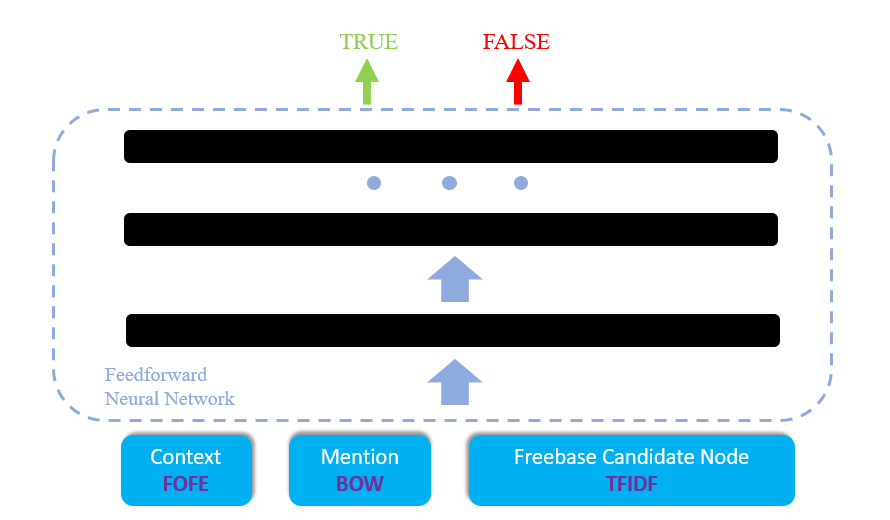
\includegraphics[width=0.7\textwidth]{FOFE-Entity-Linking.png}\\
  \caption{Our Entity Linking system use FOFE features as input and a feed-forward neural network as model.}\label{FOFE-DL-fg:2}
\end{figure*}

We recognize that the final linking performance relies heavily  on the generated candidate list. In this
work, we utilize a rule-based system, similar to \cite{kbp2016iflytek}, as our candidate generation module to generate
candidates for each detected mention. Candidates
are generated based on knowledge bases,
including Freebase and Wikipedia. The output of
this module is a candidate list, consisting of a list
of Freebase nodes possibly matching this mention.

The candidate list for each detected mention contains
the Freebase node IDs that match with the
mention in the candidate generation process. In
this work, we propose to use a feedforward fully connected
NN ranking model to assign probabilities
to all candidates in the list. The candidate
with the highest probability is chosen as the final
linking result. Each time, our FOFE ranking model
takes the mention and a candidate from the list
to compute a score, as shown in Figure \ref{FOFE-DL-fg:2}. For each pair of the detected mention and a candidate Freebase node, we use FOFE and bag-of-words to generate fixed-size features.

\subsection{Nil Entity Clustering}

For all mentions identified as NIL by the above NN ranking models, we perform a very simple
rule-based algorithm to cluster them: Different named NIL mentions are grouped into one cluster
only if their mention strings are the same (case-insensitive).

\section{Experimental Results}

The trilingual EDL task is extended to detect nominal mentions of all 5 entity types for all three languages. In our experiments, for simplicity, we simply treat nominal mention types as some extra entity types and detect them along with named entities together with a single model.  
In the following, we will report our performance on the KBP2017  trilingual EDL track. 

\subsection{Training Data}

We make use of the following datasets as our training data to learn the NER and mention detection models. 

\begin{itemize}
	\item \textbf{Training and evaluation data in KBP2015}: In the KBP 2015 competition, 335 English documents, 313 Chinese documents and 296 Spanish documents were annotated for training and evaluation, totalling 944 documents. In this data set, all five named mention types (PER, ORG, GPE, LOC, FAC) and only one nominal mention type (PER) are labelled. 
	
	\item \textbf{Evaluation data in KBP2016}: In this data set, all five named mention types (PER, ORG, GPE, LOC, FAC) and their nominal mention type (PER) are labelled. 
	
	\item \textbf{iFLYTEK's in-house dataset}: The iFLYTEK Research has generously shared with us about 10,000 in-house English and Chinese labeled documents \cite{kbp2016iflytek}.  These documents are internally labelled by iFLYTEK using some annotation rules similar to the KBP 2016 guidelines.
	
\end{itemize}

\subsection{Multi-task Learning Results}

In our experiments, we treat the KBP EDL task as the main task for all three languages. The KBP2015 and KBP2016 datasets are used as training data for the KBP EDL task. For each language, we set up three multi-task models that are trained and evaluated independently. 

For the English model, we make use of the CoNLL-2003 and OntoNotes 5.0 datasets as auxiliary tasks. The CoNLL-2003 dataset \cite{TjongKimSang:2003:ICS:1119176.1119195} consists of newswire data originated from the Reuters RCV1 corpus. It is tagged with four entity types: person (PER), location (LOC), organization (ORG) and miscellaneous (MISC). The OntoNotes 5.0 dataset consists of text from sources such as broadcast conversation and news, newswire, telephone conversation, magazine and web text. This dataset was assembled by \cite{pradhan-etal:2013:conll-2013} for the CoNLL-2012 shared task, who specifies a standard train, validation, and test split followed in our evaluation. It is tagged with eighteen entity types, some of which are: person, facility, organization, product, data, time, money, quantity and so forth. The model has two hidden layers in the shared module and one hidden layer in the main task’s private module. The hidden layers each contain 512 units and are trained with the Stochastic Gradient Descent optimizer using mini-batch of size 256 for 128 epochs. The only form of regularization used is dropout \cite{Srivastava:2014:DSW:2627435.2670313} with a probability of 0.5. A learning rate is set to 0.128 with a decay factor of 1/16 if the validation performance drops. The loss function used is categorical cross entropy. We set the forgetting factor to $\alpha = 0.5$. We use three sets of word embeddings of 256 dimensions from the English, Spanish and Chinese gigawords for the three models. 
The Spanish and Chinese models only utilize the DAFT Light ERE dataset as the auxiliary task. The DEFT Light ERE dataset consists of discussion forum and newswire documents tagged with five types of named entities: person, title, organization, geopolitical entities and location. The setup for both languages is similar to the English model, except the learning rate used is 0.064, with mini-batch of size 128. Also, the Spanish model contains a single hidden layer in the shared module. 
We combine our in-house dataset to KBP2017 training data for the English and Chinese models. 

We have evaluated the above multi-task learning (MTL) method for KBP2016 evaluation data set and significant gains are observed for all three languages. The final (MTL) performance in the KBP2017 official evaluation is shown in Table \ref{tbl:summary-kbp2017-EDL4}.

\begin{table*}
	\centering
	\begin{tabular}{|c|c|c|c|}
		\hline
		LANG  &  Training data   &  Auxiliary tasks  &  $F_1$ \\ \hline \hline
			ENG &   KBP2015 (English) + in-house & CoNLL2003, OntoNotes 5.0 & 0.780 \\
			CMN  &  KBP2015 (Chinese) + in-house  & DEFT Light ERE Chinese & 0.685 \\	
			SPA &  KBP2015 (Spanish) & DEFT Light ERE Spanish & 0.767 \\
      \hline
	\end{tabular}
	\caption{Summary of the training data and auxiliary tasks used for the entity discovery performance in KBP2017 EDL evaluation. }
	\label{tbl:summary-kbp2017-EDL4}	
\end{table*}


\subsection{Model Ensemble Results}

We have trained 4 sets of \textbf{FOFE-NER} models \cite{xu2017local,xu2016fofe,xu2016yorknrm}.
They differ in terms of initial word embedding and training data, as listed in Table \ref{tbl:model-diff}. 
Each set consists of 5 models that are cross-validated, which totals 20 models. For each model set, data is divided into 5 disjoint partitions. Each model within the same set holds out one different partition and is trained with the rest. 

The final result is produced by hard voting where 6 models agree \cite{breiman1996bagging}. 
More precisely, we treat the labels as 4-element tuples of (filename, offsets, entity-type, named-or-nominal).
Occurrences of each label are accumulated while each occurrence contributes to one voting score. If a label receives more than 6 votes out of 20, it is included in the final submission. As shown in Table \ref{tbl:kbp2017-EDL-modelensemble}, the model ensemble has significantly improved the entity discovery (ED) performance for all three languages, about 1.5\% gain in $F_1$ scores. 

\begin{table*}
	\centering
	\begin{tabular}{|l|l|l|}
		\hline
		& Embedding & Training Data \\
		\hline
		set1 & fofe-embedding & KBP2015, KBP2016, in-house  \\
		set2 & fofe-embedding & KBP2016, in-house  \\
		set3 & word2vec & KBP2015, KBP2016, in-house  \\
		set4 & word2vec & KBP2016, in-house  \\
		\hline
	\end{tabular}
	\caption{Four different sets of ED models are trained for ensemble.}
	\label{tbl:model-diff}
\end{table*}

\begin{table*}
	\centering
	\begin{tabular}{|c|c|c|c|c|c|c|}
		\hline
		LANG  &  \multicolumn{3}{|c|}{single model} & \multicolumn{3}{|c|}{model ensemble} \\ \hline
		  &  P   &  R  &  $F_1$ &  P   &  R  &  $F_1$ \\ \hline 
		ENG &  0.801 & 0.745 & 0.772 & 0.796 & 0.779 & {\bf 0.787} \\
		CMN  &  0.775 & 0.660 & 0.713 & 0.796 & 0.673 & {\bf 0.729}  \\	
		SPA &  0.856 & 0.715 & 0.779 & 0.834 & 0.762 & {\bf 0.797}  \\ \hline
		ALL & -  & -  &  - & 0.808 & 0.729 & {\bf 0.767} \\
      \hline
	\end{tabular}
	\caption{Entity Discovery (ED) performance of model ensemble in the KBP 2017 trilingual EDL evaluation. }
	\label{tbl:kbp2017-EDL-modelensemble}	
\end{table*}

\subsection{Entity Linking Results}

We have compared the FOFE-based entity linker with our two baseline systems described above. The performance comparison is shown in Table \ref{tbl:kbp2017-entity-linking}. The proposed FOFE-based entity linker has achieved similar performance as our two baseline systems, one using handcrafted features and the other using online search engines. 

\begin{table*}
\centering
\begin{tabular}{|c|c|c|c|c|c|c|}  \hline
LANG  &  \multicolumn{2}{|c|}{baseline1} & \multicolumn{2}{|c|}{baseline2} &  \multicolumn{2}{|c|}{FOFE-EL} \\ \hline
 &  NERLC  & CEAFmC  &  NERLC  & CEAFmC &  NERLC  & CEAFmC \\ \hline
ENG &  {\bf 0.646} & 0.630 &  0.572 & 0.615 & 0.604 & {\bf 0.646} \\
CMN  &  {\bf 0.617} & {\bf 0.650} & 0.579 & 0.615 & 0.487 & 0.635 \\	
SPA  & {\bf 0.569} & 0.568 & 0.538 & 0.547 & 0.502 & {\bf 0.572}  \\ \hline
ALL  & {\bf 0.611} & {\bf 0.607} & 0.565 & 0.586 & - & - \\ \hline
\end{tabular}
\caption{Performance on the KBP2017 EDL evaluation of our three entity linking systems. ({\em NERLC} denotes for {\em strong\_typed\_all\_match} and {\em CEAFmC} for {\em typed\_mention\_ceaf}) } 
\label{tbl:kbp2017-entity-linking}	
\end{table*}

\section{Conclusions}

In this paper, we have described the techniques used for KBP2017 evaluation of Trilingual EDL Track. We have investigated a new FOFE-based local detection based approach for both entity discovery and linking. This method has relied on the recent fixed-size ordinally forgetting encoding (FOFE) method to fully encode each fragment and its left/right contexts into a fixed-size representation, and a simple feedforward neural network to reject or predict entity labels for each individual fragment. Using this method, our systems have achieved a strong performance in the official KBP2017 trilingual EDL evaluations. 

\bibliography{fofe4ner}
\bibliographystyle{acl2016}

\end{document}
